%-----------------------------------LICENSE------------------------------------%
%   This file is part of Mathematics-and-Physics.                              %
%                                                                              %
%   Mathematics-and-Physics is free software: you can redistribute it and/or   %
%   modify it it under the terms of the GNU General Public License as          %
%   published by the Free Software Foundation, either version 3 of the         %
%   License, or (at your option) any later version.                            %
%                                                                              %
%   Mathematics-and-Physics is distributed in the hope that it will be useful, %
%   but WITHOUT ANY WARRANTY; without even the implied warranty of             %
%   MERCHANTABILITY or FITNESS FOR A PARTICULAR PURPOSE.  See the              %
%   GNU General Public License for more details.                               %
%                                                                              %
%   You should have received a copy of the GNU General Public License along    %
%   with Mathematics-and-Physics.  If not, see <https://www.gnu.org/licenses/>.%
%------------------------------------------------------------------------------%

% Use the standalone class for displaying the tikz image on a small PDF.
\documentclass[crop, tikz]{standalone}

% Needed for mathbb.
\usepackage{amssymb}

% Import the tikz package to use for the drawing.
\usepackage{tikz}

% Load the arrows.meta library.
\usetikzlibrary{arrows.meta}

% Begin the document.
\begin{document}

    % Draw the figure.
    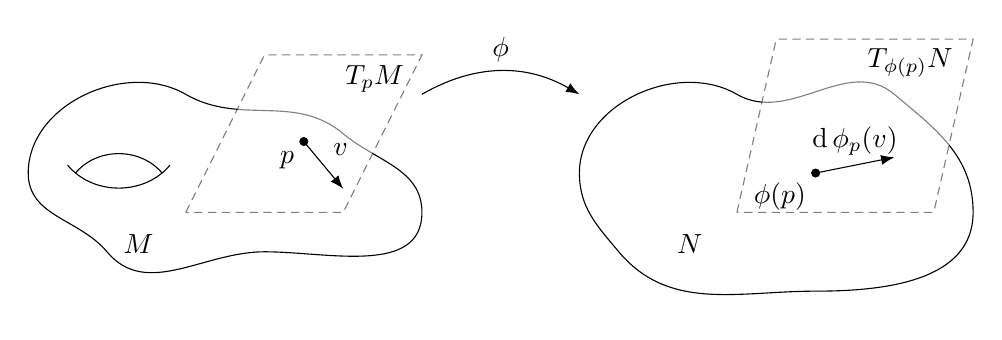
\begin{tikzpicture}[>=LaTeX]
        \coordinate (p)  at (3.5,  0.4);
        \coordinate (p1) at (4.0, -0.2);
        \draw (0.0, 0.0)    to[out=90,  in=150]  (2.0,  1.0)
                            to[out=-30, in=140]  (4.0,  0.5)
                            to[out=-40, in=90]   (5.0, -0.5)
                            to[out=-90, in=0]    (3.0, -1.0)
                            to[out=180, in=-50]  (1.0, -1.0)
                            to[out=130, in=-90]  cycle;

        \draw (0.5, 0.1) to[in=-130, out=-50] (1.8, 0.1);
        \draw (0.6, 0.0) to[in=130,  out=50]  (1.7, 0.0);
        \draw[fill=white, densely dashed, opacity=0.5]
            (2, -0.5) to (3.0,  1.5) to (5.0,  1.5)
                      to (4.0, -0.5) to cycle;

        \node at (1.4, -0.9) {$M$};
        \node at (4.4,  1.2) {$T_{p}M$};
        \draw[fill=black] (3.5, 0.4) circle (0.5mm);
        \draw[->] (p) to node[above right] {$v$} (p1);
        \node at (p) [below left] {$p$};

        \draw[->] (5, 1) to[out=30, in=150] node[above] {$\phi$} (7, 1);
        \begin{scope}[xshift=7cm]

            \coordinate (fp)  at (3.0, 0.0);
            \coordinate (fp1) at (4.0, 0.2);
            \draw (0.0, 0.0)    to[out=90,  in=150]  (2.0,  1.0)
                                to[out=-30, in=140]  (4.0,  1.0)
                                to[out=-40, in=90]   (5.0, -0.5)
                                to[out=-90, in=0]    (3.0, -1.5)
                                to[out=180, in=-50]  (0.5, -1.0)
                                to[out=130, in=-90]  cycle;

            \draw[fill=white, densely dashed, opacity=0.5]
                (2, -0.5) to (2.5,  1.7) to (5.0,  1.7) to (4.5, -0.5) to cycle;

            \node at (1.4, -0.9) {$N$};
            \node at (4.2,  1.4) {$T_{\phi(p)}N$};
            \draw[fill=black] (fp) circle (0.5mm);
            \draw[->] (fp) to node[above] {$\textrm{d}\,\phi_{p}(v)$} (fp1);
            \node at (fp) [below left] {$\phi(p)$};
        \end{scope}
    \end{tikzpicture}
\end{document}
